We are using GitHub Actions to automate the testing and deployment of Minitwit. There are 5 GitHub Actions workflows:

\begin{outline}[enumerate]
    \1 Deploy services to DigitalOcean
        \2 Runs when there is a push to \code{main}.
        \2 This workflow builds and pushes Docker images to Docker Hub, and then pulls them to the server on DigitalOcean.
    \1 Run tests and linter
        \2 Runs on any push or when a PR is updated/created.
        \2 Runs linters and tests on new commit or PR.
    \1 Release MiniTwit
        \2 Runs every thursday at 23:30 UTC.
        \2 Creates a weekly release of MiniTwit.
    \1 Run linter
        \2 Runs when called by other workflows.
        \2 Lints Go files using golangci-lint.
    \1 Hadolint on dockerfiles
        \2 Runs when called by other workflows.
        \2 Lints Docker files using Hadolint.
\end{outline}
\begin{figure}[H]
    \centering
    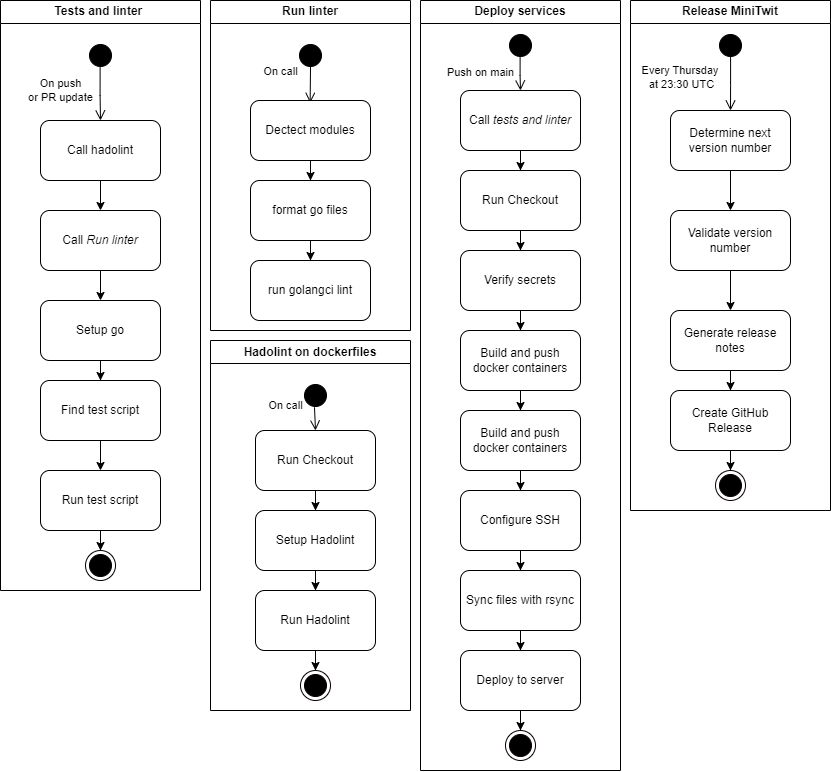
\includegraphics[width=\textwidth]{images/Worflows.png}
    \caption{Activity diagram of the workflows.}
\end{figure}
